\phantomsection
%\addcontentsline{toc}{chapter}{Introduzione}
\chapter{GreenCloud Simulator Overview}
\markboth{GreenCloud Simulator Overview}{}
% [titolo ridotto se non ci dovesse stare] {titolo completo}

\begin{citazione}

\end{citazione}
\newpage

\section{Selection of GreenCloud} 
Based on the comparisons made among the different analyzed simulators, each of them has its strengths and weaknesses. However, for the needs required in the study addressed by this thesis work, it is essential to prioritize aspects related to the energy consumption of the computing center and the accuracy of simulations. From the conducted comparisons, it is evident that \emph{GreenCloud} is the simulator that accurately considers these aspects as it is built on top of \emph{NS2} simulator and fully implements the \emph{TCP/IP} protocol. Moreover, \emph{GreenCloud} offers its users a set of features related to the simulation and to the energy consumption management. In particular, it is possible to choose between several pre-implemented Data Center architectures and energy models as well as to customize them. Furthermore \emph{GreenCloud} provides various workload scheduling and power saving models, allowing programmers to implement new ones. Despite \emph{GreenCloud} simulation times tend to be high, for the purposes of this study it is reasonable to prioritize granularity over performance. Therefore, the study will continue using \emph{GreenCloud} as the reference tool for the simulations to be conducted.


\section{Available Data Center architectures}
As mentioned in the previous section, \emph{GreenCloud} provides several Data Centers architectures. The implemented architectures consist of various components, described as follows:
\begin{itemize}
    \item \textbf{Servers: } single core nodes with a fixed processing power limit expressed in \emph{MIPS} (million instructions per second) or \emph{FLOPS} (floating point operations per second) that are responsible for task execution. These components are organized in racks and the architecture includes the presence of a Top-of-Rack switch that connects them to the access layer of the architecture;
    \item \textbf{Switches and links: } they implement the interconnection between the Servers in the Data Center. The type and the quality of these devices influences the transmission rate, anyway the costs of such devices need to be taken into account. Switches usually support either 1 \emph{GE (Gigabit Ethernet)} or 10 \emph{GE} as transmission rates, while links usually support 10 \emph{Mb/s}, 100 \emph{Mb/s}, and 1 \emph{Gb/s} as transmission rates;
    \item \textbf{Workloads: } the representation of tasks to be executed that consist of two components, computational and communicational. The computational part specifies the required amount of computing resources, measured in \emph{MIPS} or \emph{FLOPS}, and the duration of resource allocation. On the other hand, the communicational component of the workload entails the quantity and dimensions of data transfers essential before, during, and after the workload execution.
\end{itemize}
The following subsections provide an overview of the available Data Center architectures within the \emph{GreenCloud} simulator.

\subsubsection{Two-tier Data Center architecture}
The two-tier architecture is shown in figure \ref{fig:greencloud_twotier}. This architecture consists of an \emph{Access Network} where rack switches group several computing Servers through 1 \emph{GE} links and a \emph{Core Network} where L3 switches provide full mesh connectivity through 10 \emph{GE} links. This type of architecture supports up to 5500 nodes.
\begin{figure}[h]
    \centering
    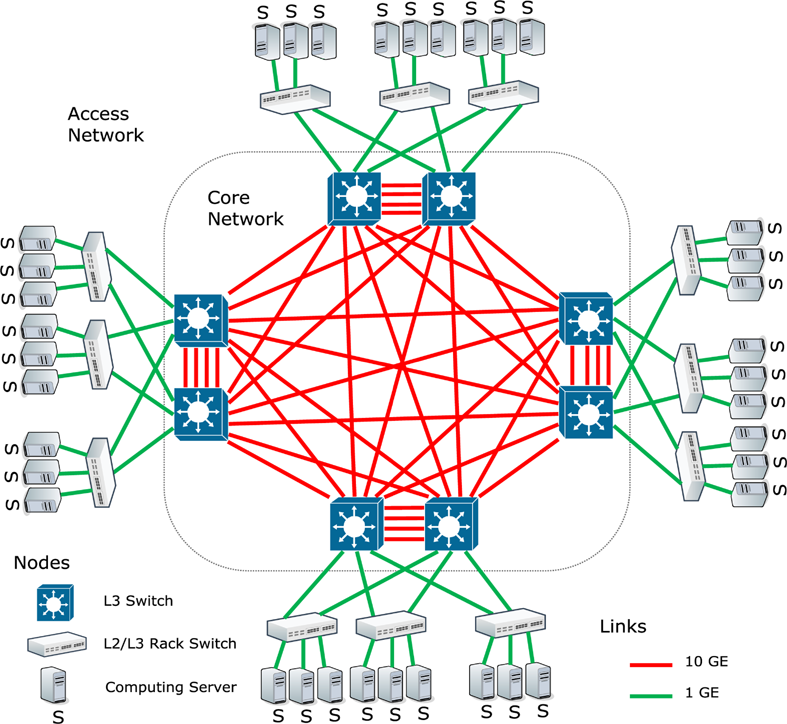
\includegraphics[width=0.5\textwidth]{chapters/images/greencloud_twotier.png}
    \caption{GreenCloud two-tier architecture}
    \label{fig:greencloud_twotier}
\end{figure}

\subsubsection{Three-tier Data Center architecture}

\section{Energy model of switches, CPU, memory and disks}

\section{Available power saving models}

\section{Workload scheduling algorithms comparison} 
    
